% !TeX encoding = UTF-8

%% ------------------------------------------------------------------------
%% Copyright (C) 2021-2023 SJTUG
%% 
%% SJTUBeamer Example Document by SJTUG
%% 
%% SJTUBeamer Example Document is licensed under a
%% Creative Commons Attribution-NonCommercial-ShareAlike 4.0 International License.
%% 
%% You should have received a copy of the license along with this
%% work. If not, see <http://creativecommons.org/licenses/by-nc-sa/4.0/>.
%%
%% For a quick start, check out src/doc/sjtubeamerquickstart.tex
%% Join discussions: https://github.com/sjtug/SJTUBeamer/discussions
%% -----------------------------------------------------------------------

\documentclass[xcolor=table,dvipsnames,svgnames,aspectratio=169]{ctexbeamer}
% 可以通过 fontset=macnew / fontset=ubuntu / fontset=windows 选项切换字体集;
% 如遇无法显示的数学符号,尝试对 ctexbeamer 文档类添加 no-math 选项;
% 写纯英文幻灯片可以改用 beamer 文档类。

\usepackage{tikz}
\usepackage[normalem]{ulem}
\usetikzlibrary{arrows}
\usepackage{amsmath}
\usepackage{graphicx}
\usepackage{hologo}
\usepackage{colortbl}
\usepackage{shapepar}
\usepackage{hyperxmp}
\usepackage{booktabs}
\usepackage{listings}
\usepackage{tipa}
\usepackage{multicol}
\usepackage{datetime2}
\usepackage{fontawesome5}
\usepackage{hyperref}

% 参考文献设置,使用 style=gb7714-2015 样式为标准顺序编码制,
% 使用 style=gb7714-2015ay 样式可以改为著者-出版年制。
% \usepackage[backend=biber,style=gb7714-2015]{biblatex}
% \addbibresource{ref.bib}

% 该行指定了图像的额外搜索路径
\graphicspath{{figures/}}

\hypersetup{
  pdfcopyright       = {Licensed under CC-BY-SA 4.0. Some rights reserved.},
  pdflicenseurl      = {http://creativecommons.org/licenses/by-sa/4.0/},
  unicode            = true,
  psdextra           = true,
  pdfdisplaydoctitle = true
}

\pdfstringdefDisableCommands{
  \let\\\relax
  \let\quad\relax
  \let\hspace\@gobble
}

% \renewcommand{\TeX}{\hologo{TeX}}
% \renewcommand{\LaTeX}{\hologo{LaTeX}}
% \newcommand{\BibTeX}{\hologo{BibTeX}}
% \newcommand{\XeTeX}{\hologo{XeTeX}}
% \newcommand{\pdfTeX}{\hologo{pdfTeX}}
% \newcommand{\LuaTeX}{\hologo{LuaTeX}}
% \newcommand{\MiKTeX}{\hologo{MiKTeX}}
% \newcommand{\MacTeX}{Mac\hologo{TeX}}
% \newcommand{\beamer}{\textsc{beamer}}
% \newcommand{\XeLaTeX}{\hologo{Xe}\kern-.13em\LaTeX{}}
% \newcommand{\pdfLaTeX}{pdf\LaTeX{}}
% \newcommand{\LuaLaTeX}{Lua\LaTeX{}}
% \def\TeXLive{\TeX{} Live}
% \let\TL=\TeXLive

% \newcommand{\SJTUThesis}{\textsc{SJTUThesis}}
% \newcommand{\SJTUThesisVersion}{2.0.3}
% \newcommand{\SJTUThesisDate}{2023/9/25}
% \newcommand{\SJTUBeamer}{\textsc{SJTUBeamer}}
% \newcommand{\SJTUBeamerVersion}{3.0.0}
% \newcommand{\SJTUBeamerDate}{2022/11/22}

% \newcommand\link[1]{\href{#1}{\faLink}}
% \newcommand\pkg[1]{\texttt{#1}}

% \def\cmd#1{\texttt{\color{structure}\footnotesize $\backslash$#1}}
% \def\env#1{\texttt{\color{structure}\footnotesize #1}}
% \def\cmdxmp#1#2#3{\small{\texttt{\color{structure}$\backslash$#1}\{#2\}
% \hspace{1em}\\ $\Rightarrow$\hspace{1em} {#3}\par\vskip1em}}

\usetheme[maxplus,blue,light]{sjtubeamer}
\setbeameroption{show notes on second screen=bottom}
% 使用 maxplus/max/min 切换标题页样式
% 使用 red/blue 切换主色调
% 使用 light/dark 切换亮/暗色模式
% 使用外样式关键词以获得不同的边栏样式
%   miniframes infolines  sidebar
%   default    smoothbars split	 
%   shadow     tree       smoothtree
% 使用 topright/bottomright 切换徽标位置
% 使用逗号分隔列表以同时使用多种选项

% \setbeamertemplate{background}{}
% 对于 max 主题,如果需要关闭正文背景图,请取消注释上一行。

% \tikzexternalize[prefix=build/]
% 如果您需要缓存 tikz 图像,请取消注释上一行,并在编译选项中添加 -shell-escape。

\lstset{
  language=[LaTeX]TeX,           % 更改高亮语言
  texcsstyle=*\color{cprimary},  % 只在高亮 LaTeX 语言时必须
  tabsize=2,
  basicstyle=\ttfamily\scriptsize,%
  keywordstyle=\color{cprimary},%
  stringstyle=\color{csecondary},%
  commentstyle=\color{ctertiary!50!gray},%
  breaklines,%
}
\logo{}
\author{熊家辉}
\institute[萨塞克斯人工智能学院]{浙江工商大学}
% \date{\the\year 年 \the\month 月}
\date{2024 年 8 月 23 日}
% \date{\today}
\subject{Arduino on Milk-V Duo}
\keywords{Arduino, RISC-V, Milk-V Duo}

\title[Arduino on Milk-V Duo] % 页脚显示标题
{\textbf{测评 Arduino 对 Milk-V Duo 适配}} % 首页标题

\subtitle{PLCT 实验室西湖开放日与香山南湖笔记本展示会}

\begin{document}

% 使用节目录
\AtBeginSection[]{
  \begin{frame}
    %% 使用传统节目录,也可以将 subsectionstyle=... 换成 hideallsubsections 以隐藏所有小节信息
    % \tableofcontents[currentsection,subsectionstyle=show/show/hide]
    %% 或者使用节页
    \sectionpage
  \end{frame}
}

% 使用小节目录
\AtBeginSubsection[]{		       % 在每小节开始
  \begin{frame}
    %% 使用传统小节目录
    % \tableofcontents[currentsection,subsectionstyle=show/shaded/hide]
    %% 或者使用小节页
    \subsectionpage
  \end{frame}
}

\maketitle

\begin{frame}
  \frametitle{自我介绍}
  % \begin{thebibliography}{00}
  %   \setbeamertemplate{bibliography item}[online]
  %   \bibitem{} Alexara Wu.
  %   \newblock 如何使用 \LaTeX{} 排版论文[EB/OL].
  %   \newblock 2021.
  %   \url{https://github.com/sjtug/sjtulib-latex-talk/tree/alexara-2021}
  % \end{thebibliography}

  % \vspace*{2ex}
  % ;;现工作于中国科学院软件研究所编程和编译语言实验室测试工程方向,在工作期间曾主管 openEuler RISC-V 主线化测试工作、中国大陆第一个 RISC-V 架构主线化支持的操作系统测试工作并代表测试团队出席与 openEuler Developer Day 2023 一同举行的 openEuler 技术委员会会议;现任珠海横琴群芯汇聚投资合伙企业(Milk-V)合伙人。参与多个知名开源项目的 RISC-V 支持建设和测试工作,包括 Numpy、openEuler、openKylin、Deepin、openWRT。曾参加 RISC-V China Summit 2023 并担任志愿者组长。持有中国业余无线电操作证,有效期内的呼号为 BG5CQH 的中华人民共和国无线电台执照(地面无线电业务);持有有效的轻型民用无人驾驶航空器安全操控理论培训合格证明。

  \begin{itemize}
    \item 熊家辉,就读于浙江工商大学萨塞克斯人工智能学院通信工程(中外合作)专业,预计于 2026 年 8 月获得浙江工商大学工学学士学位和萨塞克斯大学荣誉工程学士学位。
    \item 在 2023 年 10 月被萨塞克斯大学信息与工程学院选举为国际学生代表(任期至 2024 年 5 月)。现工作于 PLCT Lab 测试团队。现任群芯闪耀(Milk-V)合伙人。(但不是该公司代表。如欲联系该公司,请至会场 A7 展台或使用\href{https://milkv.io/}{官网}。)
    \item 曾参加 RISC-V China Summit 2023 并担任志愿者。现参加 RISC-V China Summit 2024 并担任机动和英语对接组志愿者。
    \item 持有中国业余无线电操作证,有效期内的呼号为 BG5CQH 的中华人民共和国无线电台执照(地面无线电业务);持有有效的轻型民用无人驾驶航空器安全操控理论培训合格证明。
    \item 发表译文一篇\href{https://mp.weixin.qq.com/s/0oge4bSOYCZCAZGXtiGRKA}{《RISC-V 对技术和创新的影响》}并被多家媒体转载。
  \end{itemize}

\end{frame}

\begin{frame}{目录}
  \tableofcontents[hideallsubsections]	% 隐藏所有小节信息
\end{frame}

\section{Arduino}

\subsection{Arduino 简介}

\begin{frame}
  \frametitle{Arduino 的开始}

  Arduino 是一家意大利开源硬件和软件公司、项目和用户社区。 他们设计和制造用于建造数字设备的单板微控制器和微控制器包。 Arduino 的硬件产品根据 CC BY-SA 获得许可,而软件根据 GNU 宽通用公共授权 (LGPL) 或 GNU 通用公共授权 (GPL) 获得许可,这意味着任何人都可以建立 Arduino 板并分卖软件。 Arduino板可以从官方网站或授权经销商购买。

  Arduino 板是使用各种微处理器和控制器设计的。 这些板配备了一组数字和模拟输入/输出 (I/O) 引脚,可连接到各种扩展板或面包板和其他电路。 该板具有串行通信接口,包括USB,也用于安装程序。 微控制器可以使用 C 和 C++ 编程语言以及标准 API(原文: Arduino Programming Language)进行编程,其灵感来自于处理语言,并与处理 IDE 的修改版本一起使用。 除了使用传统的编译工具链外,Arduino项目还提供了集成开发环境(IDE)和用Go语言开发的命令行工具。

\end{frame}

\begin{frame}
  \frametitle{Arduino 硬件}

    \begin{figure}
    \centering
    \begin{stampbox}
      \includegraphics
      [height=.4\textheight]
      {figures/ArduinoUnoR3.jpg}
    \end{stampbox}
    \caption{Arduino Uno R3}
  \end{figure}
\end{frame}

\begin{frame}
  \frametitle{Arduino IDE}

  Arduino IDE 支持 Windows、Linux、macOS 三种操作系统,根据您使用的系统到 \href{https://www.arduino.cc/en/software}{Arduino 官方网站} 下载对应安装包进行安装,当前最新的版本为 2.3.2,建议使用最新版本。

    \begin{figure}
    \centering
    \begin{stampbox}
      \includegraphics
      [height=.3\textheight]
      {figures/duo-arduino-02_zh.jpg}
    \end{stampbox}
    \caption{Arduino IDE 2.3.2}
  \end{figure}
\end{frame}

\begin{frame}
  \frametitle{Arduino on Milk-V Duo}

  Milk-V Duo 系列已经支持 Arduino 开发,您可以直接使用 Arduino IDE,进行简单的配置后即可使用。

  Duo 系列 CPU 采用大小核设计,Arduino 固件运行在小核中,大核负责与 Arduino IDE 通讯,接收 Arduino 固件并将其加载到小核中运行。同时,大核中的 Linux 系统也是正常运行的。

  最近一次可用的 Arduino 版本为 \href{https://github.com/milkv-duo/duo-buildroot-sdk/releases/tag/Duo-V1.1.2}{Duo-V1.1.2}。由于该版本将 RNDIS 替换为 CDC-NCM,尚未在 Windows 上提供驱动。

  该报告基于 \href{https://github.com/milkv-duo/duo-buildroot-sdk/releases/tag/Duo-V1.0.9}{Duo-V1.0.9} 完成。
\end{frame}

\section{Arduino 支持情况}

\subsection{Arduino 实现情况}

\begin{frame}
  \frametitle{Arduino on Milk-V Duo API 情况}

  Milk-V Duo 已经支持部分 Arduino API 函数。

  \begin{itemize}
    \item Digital I/O
    \item Analog I/O
    \item Wire (I2C)
  \end{itemize}

  \note{数字读写和设置模式(就是GPIO的高低电平),Analog I/O(模拟PWM的读写)和I2C读写}
\end{frame}

\begin{frame}
  \frametitle{Arduino on Milk-V Duo 支持的功能}

  Milk-V Duo 已经支持部分 Arduino 功能。

  \begin{itemize}
    \item GPIO
    \item UART
    \item I2C
    \item SPI
    \item PWM
    \item ADC
  \end{itemize}

  % \note{数字读写和设置模式(就是GPIO的高低电平),Analog I/O(模拟PWM的读写)和I2C读写}
\end{frame}

\subsection{数字类驱动}

\begin{frame}
  \frametitle{Arduino GPIO on Milk-V Duo}

  GPIO 即 Digital I/O,可用于驱动数字类外设,如 DHT22。GPIO 只有高电平和低电平。

  \begin{figure}
    \centering
    \begin{stampbox}
      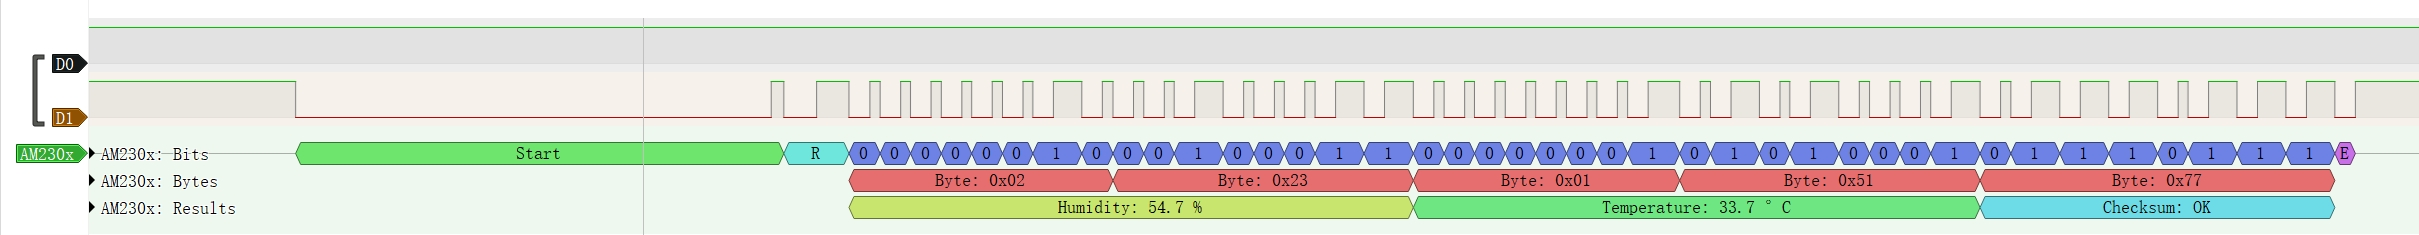
\includegraphics
      [height=.3\textheight]
      {figures/DHT22.png}
    \end{stampbox}
    \caption{DHT22 Wave}
  \end{figure}

  % \note{数字读写和设置模式(就是GPIO的高低电平),Analog I/O(模拟PWM的读写)和I2C读写}
\end{frame}

\begin{frame}[fragile,allowframebreaks]
  \frametitle{Arduino UART on Milk-V Duo}

  通用异步收发传输器是一种异步收发传输器,是电脑硬件的一部分,将数据通过串列通信进行传输。UART通常用在与其他通信接口的连接上。 具体实物表现为独立的模块化芯片,或是微处理器中的内部周边设备。UART 也依赖 GPIO。

  UART 串口默认使用的是物理引脚 6/7 上的 UART3,在调试 Arduino 程序时,可以通过该串口打印调试信息。

  部分线缆可能无法承载较高的波特率。

  \newpage

  \begin{codeblock}{UART 封装}
void setup() {
  Serial.begin(38400);
}
void loop() {
  Serial.printf("hello world\r\n");
  delay(1000);
}
\end{codeblock}
\end{frame}

\begin{frame}
  \frametitle{Arduino I2C on Milk-V Duo}

  I2C 是一种串行通信总线,使用多主从架构,由飞利浦公司在1980年代为了让主板、嵌入式系统或手机用以连接低速周边设备而发展。常用于驱动 SSD1306 等设备。可以使用 \lstinline|i2cdetect| 检测 I2C 设备。

  \begin{figure}
    \centering
    \begin{stampbox}
      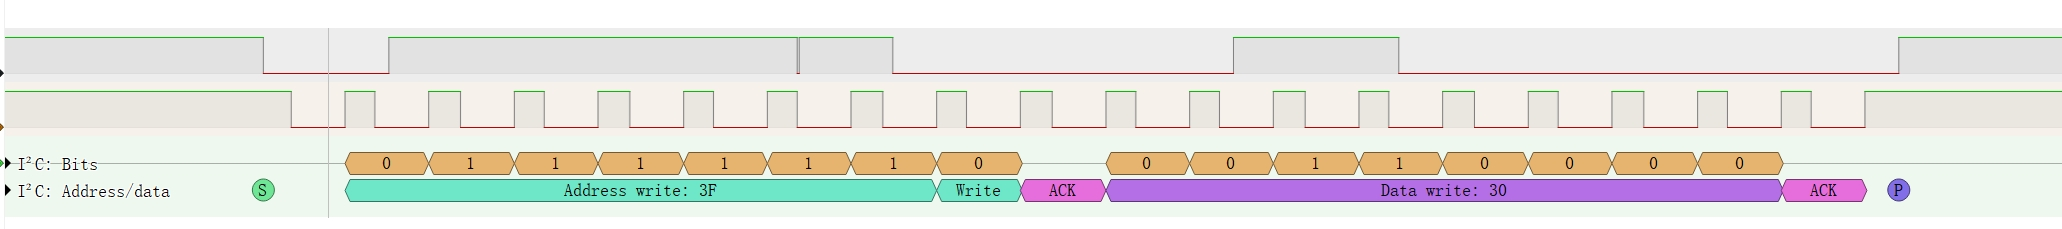
\includegraphics
      [height=.1\textheight]
      {figures/1602wave.png}
    \end{stampbox}
    \caption{LCD1602 Wave}
  \end{figure}

\end{frame}

\begin{frame}
  \frametitle{Arduino SPI on Milk-V Duo}

  SPI 是串行外设接口,是一种用于芯片通信的同步串行通信接口规范,主要应用于单片机系统中的信号传递。%类似的技术还有I²C等。 摩托罗拉公司于20世纪80年代中期首先开发出此传输接口,之后逐渐发展为行业规范之一。它的典型应用有闪存、EEPROM、SD卡与液晶显示器。

  \note{需要硬件连接如下,将 I2C1 和 I2C2 的 SDA 和 SCL 引脚对应连接,再按上述 UART 示例中的方法连接串口到电脑上查看打印信息。}

\end{frame}

\subsection{模拟类驱动}

\begin{frame}
  \frametitle{Arduino PWM on Milk-V Duo}

  脉冲宽度调制,简称脉宽调制,是用脉冲来输出模拟信号的一种技术,一般变换后脉冲的周期固定,但脉冲的工作周期会依模拟信号的大小而改变。 在模拟电路中,模拟信号的值可以连续进行变化,在时间和值的幅度上都几乎没有限制,基本上可以取任何实数值,输入与输出也呈线性变化。

  PWM 可以驱动蜂鸣器。

  \begin{figure}
    \centering
    \begin{stampbox}
      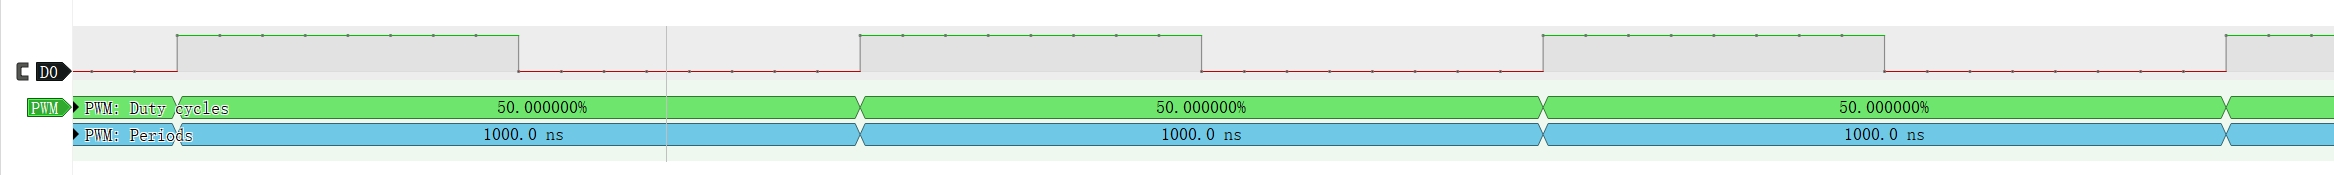
\includegraphics
      [height=.2\textheight]
      {figures/PWM.png}
    \end{stampbox}
    \caption{PWM Wave}
  \end{figure}

\end{frame}

\begin{frame}
  \frametitle{Arduino ADC on Milk-V Duo}

  模拟数字转换器(英语:Analog-to-digital converter, ADC, A/D 或 A to D)是用于将模拟形式的连续信号转换为数字形式的离散信号的一类设备。一个模拟数字转换器可以提供信号用于测量。与之相对的设备成为数字模拟转换器。

  典型的模拟数字转换器将模拟信号转换为表示一定比例电压值的数字信号。

\end{frame}

\makebottom

\end{document}